%\documentclass{article}
%\usepackage[spanish]{babel}
%\usepackage{amssymb, amsmath} %Paquetes matemáticos de la American Mathematical Society
%\usepackage{graphicx}
%\usepackage[%
%    a4paper,       % Tamaño de papel
%    left=2.5cm,    % Margen izquierdo
%    right=2.5cm,   % Margen derecho
%   top=3cm,       % Margen superior
%    bottom=3cm,    % Margen inferior
%    footskip=1.5cm % Espacio para el pie de página
%]{geometry}
%\usepackage{fancyhdr}
%\pagestyle{fancy}
%\fancyhf{}
%\lhead[\leftmark]{Síntesis de Redes Activas - Laboratorio 1}
%\rfoot[]{\thepage}
%\begin{document}
 \section{Circuito IV: COMPARADOR CON HISTÉRISIS}

\subsection{Esquemático y datos}

Se realiza el análisis teórico del circuito que se muestra en la siguiente figura: 
 \vspace{1em}

  \begin{figure}[h!]
     \centering
	 \includegraphics[width=0.4\linewidth]{esquematico4.png}
	 \caption{Esquematico del circuito N° 4}
	 \label{fig:esquematico4}
  \end{figure}
  
  \vspace{1em}
Este se trata de un circuito Schmitt Trigger inversor implementando un AO.

\textbf{Datos:}

\begin{itemize}
  \item Amplificador operacional LM324
  \item $V^+ = 10 \, \text{[V]}$
  \item $V^- = 0 \, \text{[V]}$
  \item $R_1 = R_2 = R_4 = 10k\Omega , R_3 = 2K\Omega$
  \item $V_{ref} = 2V $
\end{itemize}

\vspace{1em}

\subsection{Análisis teórico}

El circuito IV consiste en un comparador con histéresis, es decir, este va a comparar las entradas no inversora e inversora y en base a esto, satura su salida a $V_{cc} $ o $ V_{ss} $ dentro de un
intervalo dado por las tensiones umbrales de conmutación. Se analiza el modo diferencial de las entradas:

\[V^- = k_1 * V_i\]
\[V^+ = k_2 * (V_o - V_{ref}) + V_{ref}\]
Con:
\[k_1 = \frac{R_2}{R_1 + R_2}\]
\[ k_2 = \frac{R_3}{R_3 + R_4}\]

\vspace{1em}

\textbf{Caso $V_d<$0}

Siendo $V_d = V^+ - V^-$ Si la tensión $V_d < 0$ y $V^+ < V^-$,  se considera que en este caso la tensión de salida tiene un valor inicial Vo=Vcc y luego pasa a tener un valor Vo=Vee, debido a la acción de conmutación.  Entonces se tiene:

\[V_d = V^+ - V^- < 0 \quad \Rightarrow \quad V_o = V_{ee}\]

\[k_2 * (V_o - V_{ref}) + V_{ref} < k_1 * V_i\]
\[\frac{k_2}{k_1} * (V_o - V_{ref}) + \frac{V_{ref}}{k_1} < V_i \]
\[\frac{k_2}{k_1} * V_o + \frac{1 - k_2}{k_1} * V_{ref} < V_i \]
Se tiene:
\[ k_1 = \frac{R_2}{R_1 + R_2} = \frac{10K\Omega}{10K\Omega + 10K\Omega} = 0.5\]

\[ k_2 = \frac{R_3}{R_3 + R_4} = \frac{2K\Omega}{2K\Omega + 10K\Omega} = 0.166\]

Reemplazando en la expresión anterior:

\[\frac{0.166}{0.5} * 10V + \frac{1 - 0.166}{0.5} * 2V < V_i \]
\[3.32V + 3.34V < V_i \]
\[V_i > 6.66V \quad \Rightarrow \quad V_o = V_{cc}\]

Siendo en este caso Vcc= 10V.

\[V_i > 6.66V \Rightarrow V_o = 10V\]

\textbf{Caso  $V_d >$0}

Se tiene que $V_d > 0$ y $V^+ > V^- $. Por lo tanto la salida tiene que ser positiva. 
Previo a esta condición, el circuito tendrá un valor de salida de Vo=Vee, por lo que conmutará de un valor de Vo=Vee a Vo= Vcc. Se desarrolla la condición planteada:

\[V_d = V^+ - V^- > 0 \quad \Rightarrow \quad V_o = V_{cc}\]

\[ k_2 * (V_o - V_{ref}) + V_{ref} > k_1 * V_i\]

\[\frac{k_2}{k_1} * V_o + \frac{1 - k_2}{k_1} * V_{ref} > V_i \]
Como Vee= 0v, se tiene:

\[\frac{0.166}{0.5} * 0V + \frac{1 - 0.166}{0.5} * 2V > V_i \]
\[\frac{1 - 0.166}{0.5} * 2V > V_i \]

\[V_i < 3.336V \Rightarrow V_o = V_{ee}\]

En este caso:

\[V_i < 3.336V \Rightarrow V_o = 0V\]

\vspace{1em}

\newpage

\subsection{Simulación: }

\vspace{1em}

Utilizando LTSpice para simular el circuito planteado, se tiene:

\vspace{1em}

 \begin{figure}[h!]
      \centering
      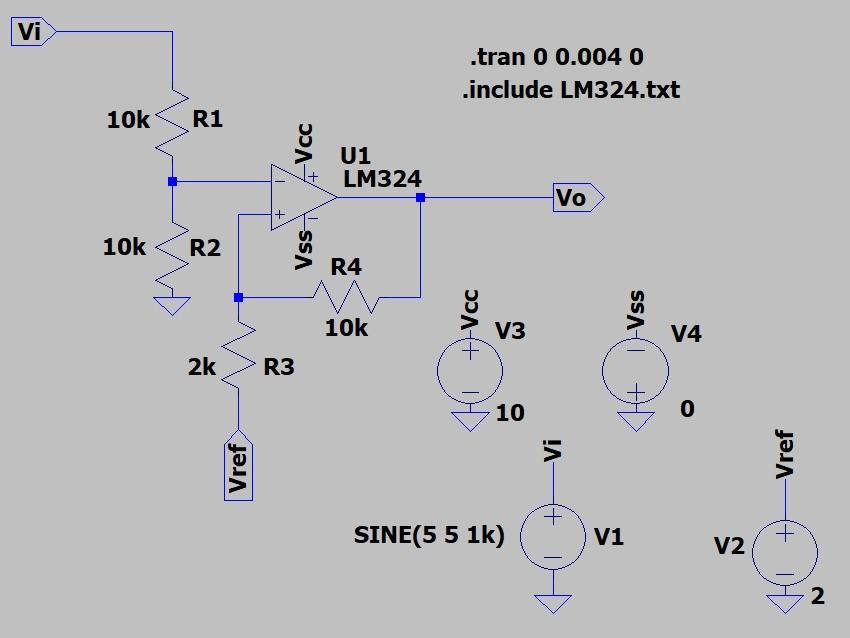
\includegraphics[width=0.4\linewidth]{simulacionC4.png}
      \caption{Simulación del circuito N° 4}
      \label{fig:simulacionC4}
 \end{figure}
 
\vspace{1em}

 \begin{figure}[h!]
        \centering
 	 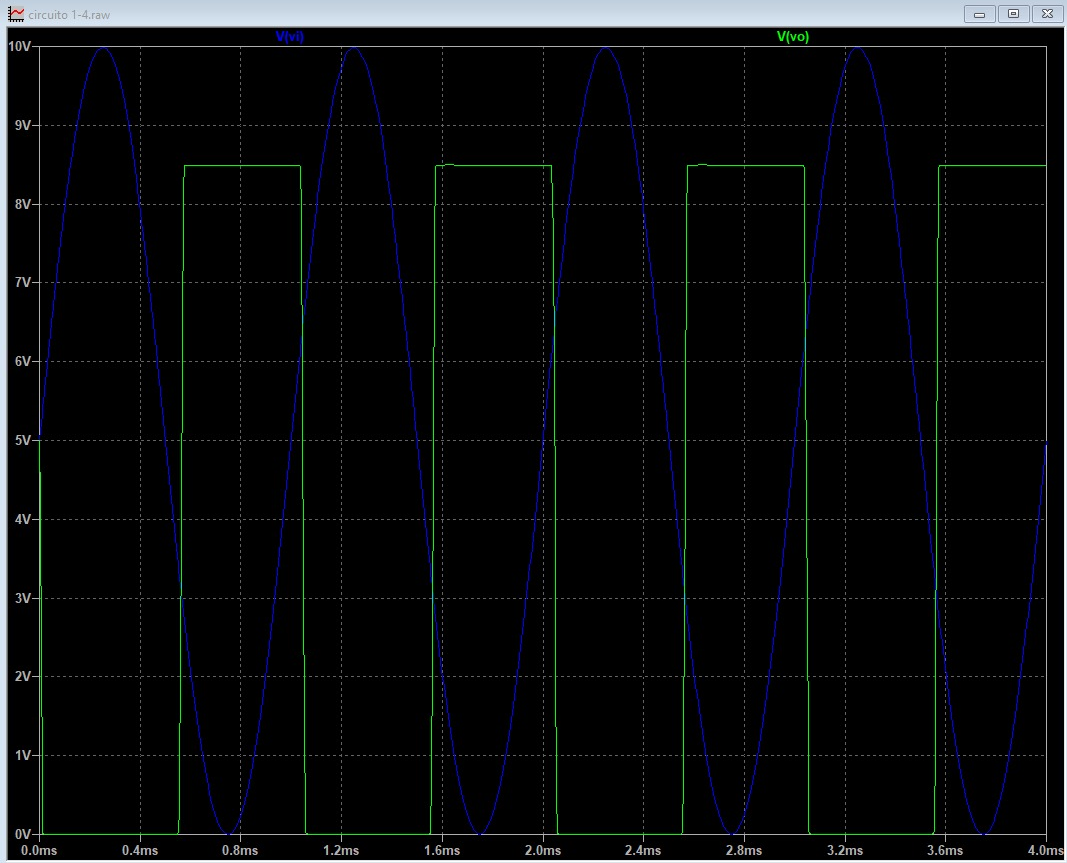
\includegraphics[width=0.5\linewidth]{c4tensionA.png}
	  \caption{Señal de salida para $V_{ss} \leq V_{in} \leq V_{cc}$}
	  \label{fig:simulacionC4}
 \end{figure}

\vspace{1em}

Haciendo una vista amplificada de las curvas se pueden apreciar mejor los valores de conmutación:

\begin{figure}[h!]
     \centering
	 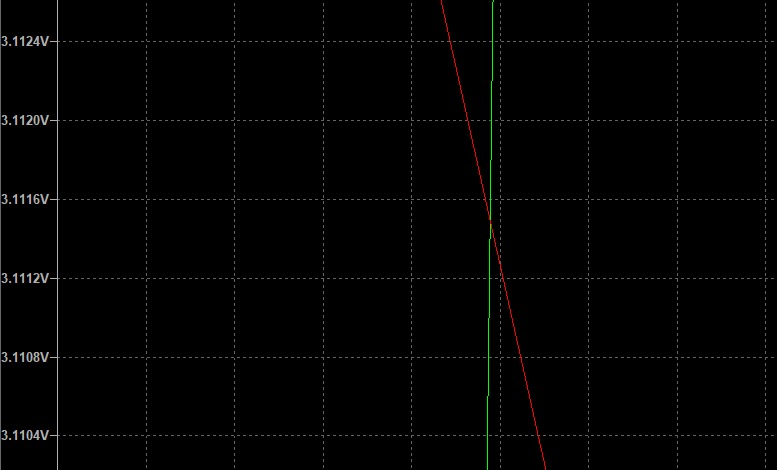
\includegraphics[width=0.4\linewidth]{c4zoomCI.png}
	 \caption{Zoom en el umbral de conmutación inferior de $V_{in} \quad y \quad V_o$}
	 \label{fig:simulacionC4}
\end{figure}

\begin{figure}[h!]
     \centering
	 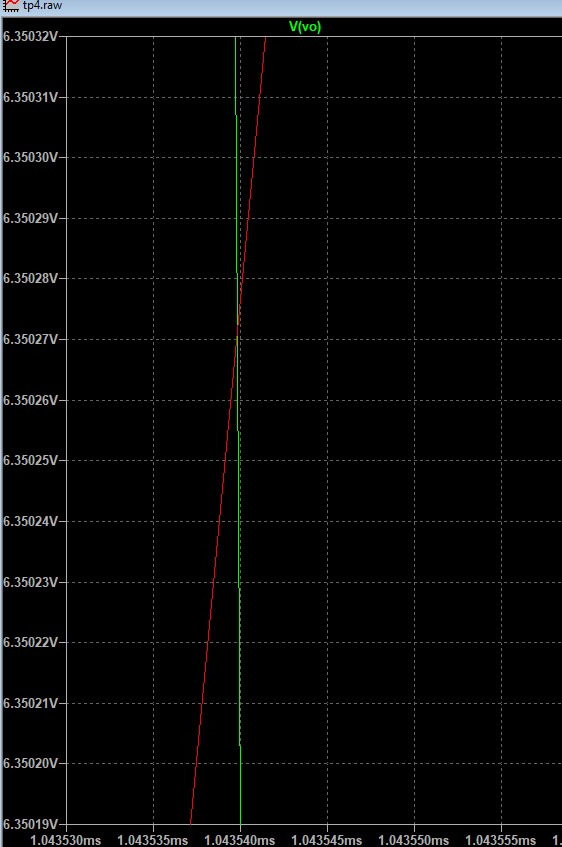
\includegraphics[width=0.4\linewidth]{c4zoomCS.png}
	 \caption{Zoom en el umbral de conmutación inferior de $V_{in} \quad y \quad V_o$}
	 \label{fig:simulacionC4}
\end{figure}


\vspace{1em}

Las imágenes de la simulación muestran el punto de intersección entre $V_{in} \quad y \quad V_o$ cumpliendo con lo planteado en el cálculo teórico.

Luego se puede observar la curva de histéresis graficando los valores de tensión $V_{in}$ y $V_o$


\vspace{1em}

\begin{figure}[h!]
     \centering
     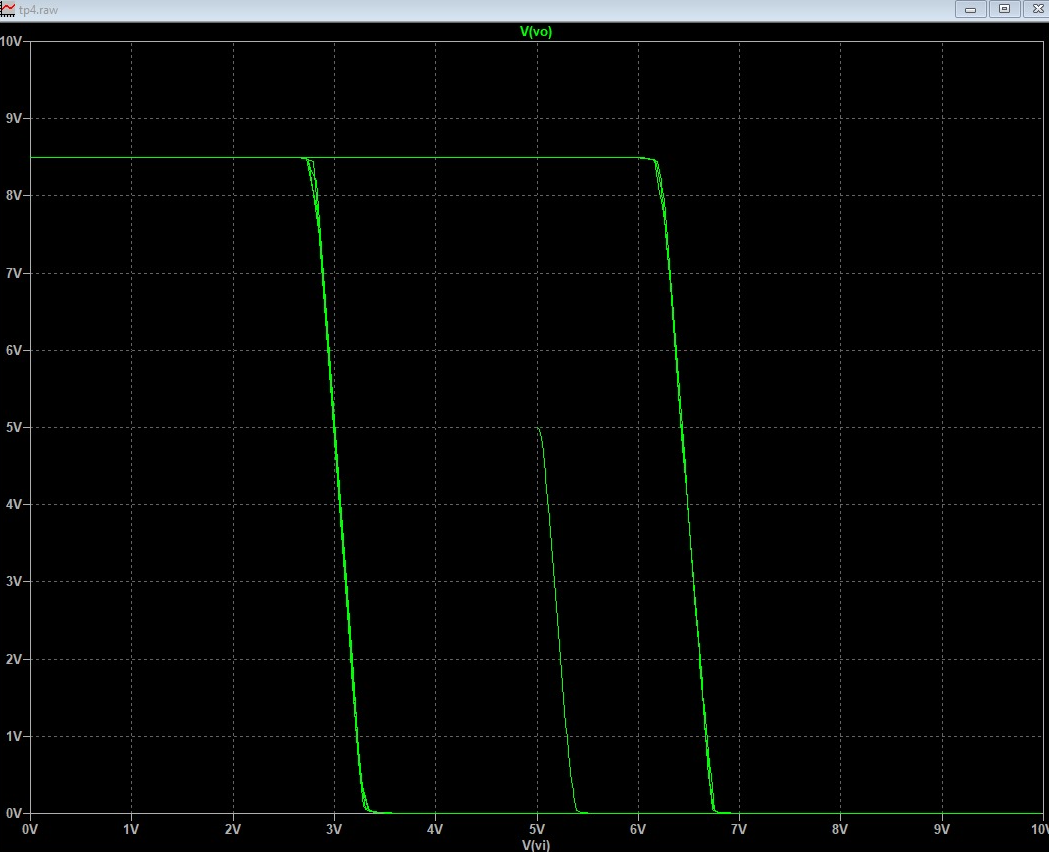
\includegraphics[width=0.5\linewidth]{c4histeresis.png}
     \caption{Curva de histéresis del comparador}
     \label{fig:simulacionC4}
\end{figure}

\vspace{1em}

Con la figura 30 queda corroborado el comportamiento característico de un comparador con histéresis. El comienzo de la señal sinusoidal se da en aproximadamente 5V y continua el trazo la curva externa 
analogamente a la histéresis de un materal ferromagnético.

\newpage

\subsection{Conclusiones}
Como conclusión a este informe se puede afirmar que se obtuvieron los resultados esperados. Comparando los valores obtenidos en el laboratorio con los obtenidos
mediante simulación y desarrollo teórico, se puede apreciar un pequeña diferencia entre los mismos. Esto se debe a que, tanto en el análisis como en la simulación se
consideran a los amplificadores operacionales como ideales, mientras que en la práctica eso no es así y existen una serie de errores que hay que tener en cuenta.

Se llegó observar claramente la no idealidad de estos amplificadores dado que ni su ganancia $A_d$, ni la relación de rechazo en modo común (RRMC) son infinitos.

También, a través de estos laboratorios se comprobró experimentalmente todo lo visto en la materia hasta el momento, tanto en la parte teórica como en la
resolución de problemas.

%\end{document}